\section{The Case for Giza}
\label{sec:motivation}

This section presents the characteristics of a large-scale cloud drive service with hundreds of millions of users. These characteristics motivate the design choices of Giza.
%The section is concluded with a discussion of an alternative approach.

\subsection{Cloud Drive Characteristics}

\begin{figure}[tp]
%\centering
\hspace{-3em}
\begin{subfigure}{.3\textwidth}
  \centering
  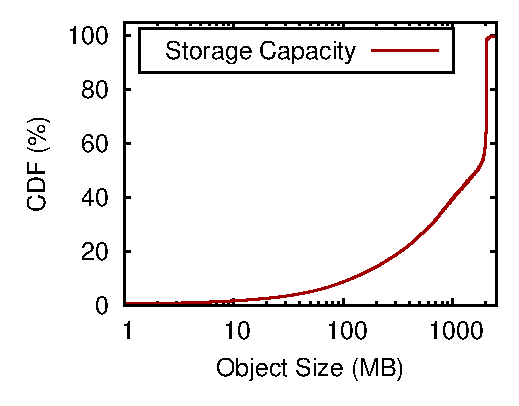
\includegraphics[width=\linewidth]{data/object_size-storage_capacity}
  \caption{}
  \label{fig:object_size-storage_capacity}
\end{subfigure}%
%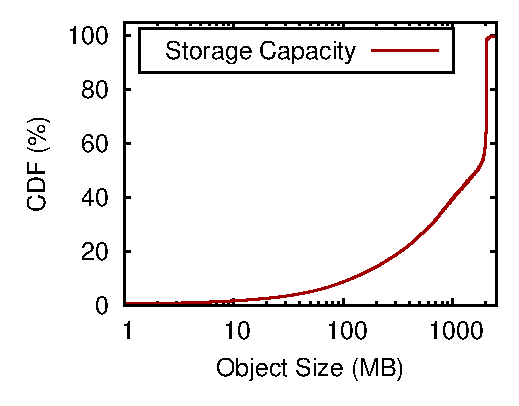
\includegraphics[width=0.5\textwidth]{data/object_size-storage_capacity}
%\hspace{-2em}
\begin{subfigure}{.3\textwidth}
  \centering
  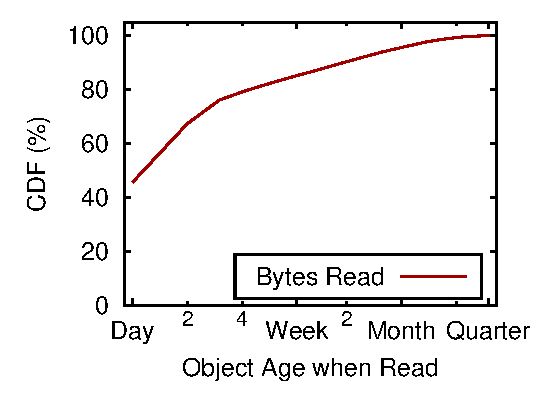
\includegraphics[width=\linewidth]{data/write_read_gap-bytes_read}
  \caption{}
  \label{fig:write_read_gap-bytes_read}
\end{subfigure}%
\caption{Cloud Drive Characteristics}
\label{fig:case_for_giza}
\end{figure}

{\bf Methodology:} The data presented in this section is derived from a three-month trace of a tier-1 cloud drive service. The cloud drive serves hundreds of millions of users and stores their objects, including documents, photos, music, videos, configuration files and more. The trace includes {\em all} reads, writes and updates to {\em all} objects between January 1 and March 31, 2016. We observe the following:

{\bf Large Objects Dominate:} The size of the objects varies significantly, ranging from Kilobytes to tens of Gigabytes. While the number of small objects vastly exceeds that of large objects, the storage capacity occupied by the small objects turns out to be small. Figure~\ref{fig:object_size-storage_capacity} presents the cumulative distribution of storage capacity consumption in terms of object size. We observe that less than $0.9\%$ of the total storage capacity is occupied by objects smaller than 4MB. This suggests that, to optimize storage cost, it is sufficient for Giza to focus on objects of 4MB and larger~\footnote{Objects of tens of Gigabytes are divided into 4MB chunks before storing in cloud storage back-end.}. Objects smaller than 4MB can simply use the existing geo-replicated storage system. This design choice reduces the overhead associated with erasure coding of small objects (including meta-data for the smaller object). As a result, all following analysis filter out objects smaller than 4MB.

{\bf Object Temperature Drops Fast:} A common usage scenario of cloud drive is sharing. Objects stored in the cloud drive are often shared across multiple devices, as well as among multiple users. Therefore, it is typical to observe reads soon after the objects are created. To this end, Figure~\ref{fig:write_read_gap-bytes_read} presents the cumulative distribution of bytes read in terms of object age when the reads occur~\footnote{The analysis focuses on all the objects created during the three-month period. Hence, the object age is capped at three months.}. It is worth pointing out that $47\%$ of the bytes read occurred in the same day of object creation, $87\%$ occurred within the same week, and merely less $2\%$ occurred beyond one month. This suggests that the temperature of the objects drops at a fast space. Moreover, caching the objects for a short period of time can satisfy most of the reads (more below).

\begin{table}[h]
\footnotesize
\centering
\begin{tabular}{|c||c|c|}
\hline \hline
total reads (B) / writes (B) 	& \multicolumn{2}{c|}{2.3$\times$}
\\ \hline \hline
%\multirow{4}{*}{cross-DC reads / writes \newline in Giza}
	& no caching		& 1.15$\times$
\\ \cline{2-3}
cross-DC reads / writes
	& caching (day)		& 0.61$\times$ 
\\ \cline{2-3}
with Giza
	& caching (week)	& 0.18$\times$ 
\\ \cline{2-3}
	& caching (month)	& 0.05$\times$ 
\\ \hline \hline
\end{tabular}
%\caption{Giza with Caching in Local DC.}
\label{tab:caching}
\end{table}
{\bf Writes Dominate with Caching:} The above table presents the effectiveness of caching. The ratio between the total amount of bytes reads to writes is 2.3$\times$. 
%This implies that on average each object is read 2.3 times. 
As illustrated in Section~\ref{sec:alternative}, Giza incurs 1x and 0.5x cross-DC network traffic in writes and reads, respectively. Hence, the ratio between cross-DC traffic due to reads and writes is $1.15\times$. Given the temperature analysis, it is most effective for Giza to additionally cache  objects for a short period of time within one single DC. Serving reads from the caching DC dramatically reduces the cross-DC traffic due to reads. Indeed, when objects are cached for one day, the cross-DC traffic attribute to reads vs writes reduces to 0.61$\times$. When objects are cached for one month, the ratio reduces to negligible 0.05$\times$, where the cross-DC traffic is completely dominated by writes.

\begin{table}[h]
\footnotesize
\centering
\begin{tabular}{c||c|c|c}
\# of Versions 	& 	1				& 2					& $\ge 3$
\\ \hline
Percentage			& $57.96\%$	& $40.88\%$	& $1.16\%$
\end{tabular}
\label{tab:version}
\end{table}
{\bf Concurrency is Rare, but Versioning is Required:} The above table presents how often objects are updated and require versioning support. We observe that $57.96\%$ of the objects are written once and never updated during the three-month period. For the remaining, $40.88\%$ of the objects are updated exactly once and merely $1.16\%$ are updated more than twice. This suggests that concurrent updates of objects are rare in Giza (albeit possible). Hence, Giza focuses and optimizes for single writer, while at the same time supports versioning. 

%\subsection{Giza: Flexible Cross-DC erasure coding }
%
%Erasure coding across geo-graphically distributed data centers is a most effective approach to reduce storage cost while achieving the fault tolerance goal of being able to survive data center failure. As Facebook's F4 system~\ref{bib:F4} has demonstrated, replacing geo-replication with cross-DC erasure coding can effectively reduce storage overhead from 3.6x to 2.1x, achieving huge savings for Facebook's 65PB of warm storage. While a fixed 2 + 1 solution works very well for Facebook's special workload, the public cloud storage desires much more flexibility. Different customers have different desirable operating points in terms of cost, durability and latency trade-off and are willing to accept different pricing for individual needs. 
%
%Giza provide completes flexibility to the customers. When a storage account is created, the customers may specify how much fault tolerance is desired at the storage account level. In addition, the customers had additional flexibility to specify which data centers are involved, so that they could constraint all the data to be in the  United States per data sovereignty requirement and regulation, or they could choose to disperse the erasure coded data across multiple continents, so that no single country could gain access to the complete data. 

%\begin{table*}[tp]
%\centering
%\begin{tabular}{|l||c||c|c|c|c||c|c|}
%\hline
				%& Geo-Replication    	& \multicolumn{4}{c||}{Giza (standard durability)}		& \multicolumn{2}{c|}{Giza (enhanced durability)}
%\\ \hline \hline
%Number of DCs 				& 2										& 3 & 4 & 5 & 6									& 5 & 6
%\\ \hline
%Erasure coding scheme & replication					& 2 + 1 & 3 + 1 & 4 + 1 & 5 + 1	& 3 + 2 & 4 + 2
%\\ \hline \hline
%Storage overhead			& 2.6x								& 1.9x & 1.7x & 1.6x & 1.5x			& 2.1x & 1.9x
%\\ \hline
%Reduction							& -										& 27\% & 35\% & 38\% & 42\%			& 19\% & 27\%
%\\ \hline \hline
%WAN traffic (put)			& 1x									& 1x & 1x & 1x & 1x 						& 1.33x & 1.25x
%\\ \hline
%WAN traffic (get)			& 0										& 0.5x & 0.67x & 0.75x & 0.8x		& 0.67x & 0.75x
%\\ \hline
%DC rebuild 						& 1x									& 2x & 3x & 4x & 5x 						& 3x & 4x
%\\ \hline \hline
%\end{tabular}
%\caption{Trade-off of storage, bandwidth and durability.}
%\label{tab:cost_benefit}
%\end{table*}

\begin{table}[tp]
\centering
\footnotesize
\begin{tabular}{|l||c||c|c|c|}
\hline
											& Geo-Rep.						& \multicolumn{3}{c|}{Giza}
\\ \hline \hline
\# of DCs 						& 2										& 3 		& 5 		& 7
\\ \hline
Erasure coding 				& -										& 2 + 1	& 4 + 1	& 6 + 1
\\ \hline \hline
Storage overhead			& 2.6									& 1.9 	& 1.6 	& 1.5
\\ \hline
{\bf Cost savings}		& -										& {\bf 27\%} 	& {\bf 38\%} 	& {\bf 42\%}
\\ \hline \hline
cross-DC traffic (put)& 1x									& 1x 		& 1x 		& 1x
\\ \hline
cross-DC traffic (get)& 0										& 0.5x 	& 0.75x & 0.83x
\\ \hline
DC rebuild 						& 1x									& 2x 		& 4x 		& 6x
\\ \hline \hline
\end{tabular}
\caption{Giza Trade-offs}
\label{tab:cost_benefit}
\end{table}


\subsection{Giza Trade-offs}
\label{sec:alternative}

Compared to geo-replication, Giza offers more flexible trade-offs in terms of storage cost and cross-DC network traffic,
as summarized in Table~\ref{tab:cost_benefit}.
% summarizes the costs and benefits of Giza at various operating points.

{\bf Storage Cost:}
To tolerate single data center failure, geo-replication incurs the storage overhead of $2\times1.3$ = 2.6 (with single DC storage overhead at 1.3).
With $k+1$ erasure coding, where $k$ ranges from 2 to 6, Giza reduces the storage overhead to between 1.9 and 1.5, increasing cost savings from 27% to 42%.
The storage cost savings come with inflated cross-DC traffic, which is examined next.

{\bf Cross-DC Traffic:} For writes, Giza does {\em not} incur more cross-DC traffic than geo-replication. Objects are uploaded to any DC and processed by Giza in the DC. With $k+1$ erasure coding, the objects are divided into $k$ data fragments, where one fragment is stored in the DC locally and the rest $k$ fragments are stored in remote DCs. Hence, the ratio between cross-DC traffic and object size is $k/k = 1$, same as geo-replication.
For reads, however, Giza incurs additional cross-DC traffic. $k$ fragments are required to serve reads, where one is from the DC locally and the rest $k-1$ from remote DCs. Hence, the ratio between cross-DC traffic and object size is $(k-1)/k$, which increases with $k$. In comparison, geo-replication serves reads entirely from the DC locally and incurs no cross-DC traffic at all.
Upon data center failure, data originally stored at the failed DC needs to be rebuilt at a new DC. Geo-replication simply replicates every object and thus incurs 1x of cross-DC traffic. In contrast, Giza relies on erasure decoding to reconstruct missing fragments, each incurring $k$ times cross-DC traffic.

{\bf Alternative Approach:} Giza stripes individual objects across multiple DCs. This design leads to cross-DC traffic when serving reads. A possible alternative is to first aggregate objects into large logical volumes (say 100GB) and then erasure code different volumes across multiple DCs to generate parity volumes. Since every object is stored in its entirety in one of the DCs, cross-DC traffic is avoided during reads.

This design works great when objects are never deleted~\cite{f4:osdi14}. However, Giza must support deletion. Deleting objects from logical volumes (and canceling them from corresponding parity volumes) would result in complex bookkeeping and garbage collection, and greatly increases engineering complexity. In comparison, the design of Giza is much simpler, specially when (with caching enabled) reads only consume a small percentage of cross-DC traffic compared to writes. 

%%% Local Variables:
%%% mode: latex
%%% TeX-master: "main"
%%% End:
